\documentclass[a4paper,12pt]{article}

%%% Работа с русским языком
\usepackage{cmap}					% поиск в PDF
\usepackage{mathtext} 				% русские буквы в формулах
\usepackage[T2A]{fontenc}			% кодировка
\usepackage[utf8]{inputenc}			% кодировка исходного текста
\usepackage[english,russian]{babel}	% локализация и переносы
\usepackage{xcolor}
\usepackage{hyperref}
 % Цвета для гиперссылок
\definecolor{linkcolor}{HTML}{799B03} % цвет ссылок
\definecolor{urlcolor}{HTML}{799B03} % цвет гиперссылок

\hypersetup{pdfstartview=FitH,  linkcolor=linkcolor,urlcolor=urlcolor, colorlinks=true}

%%% Дополнительная работа с математикой
\usepackage{amsfonts,amssymb,amsthm,mathtools} % AMS
\usepackage{amsmath}
\usepackage{icomma} % "Умная" запятая: $0,2$ --- число, $0, 2$ --- перечисление

%% Номера формул
%\mathtoolsset{showonlyrefs=true} % Показывать номера только у тех формул, на которые есть \eqref{} в тексте.

%% Шрифты
\usepackage{euscript}	 % Шрифт Евклид
\usepackage{mathrsfs} % Красивый матшрифт

%% Свои команды
\DeclareMathOperator{\sgn}{\mathop{sgn}}

%% Перенос знаков в формулах (по Львовскому)
\newcommand*{\hm}[1]{#1\nobreak\discretionary{}
{\hbox{$\mathsurround=0pt #1$}}{}}
% графика
\usepackage{graphicx}
\graphicspath{{pictures/}}
\DeclareGraphicsExtensions{.pdf,.png,.jpg}
\author{Бурмашев Григорий, БПМИ-208}
\title{Матан, дз -- 8}
\date{\today}
\begin{document}
\maketitle
\section*{Номер 1}
Сразу говорим что $a_0 = a_k = 0$, т.к функция нечетная, а $b_k$:
\[
b_k = \frac{1}{\pi} \int\limits_{-\pi}^{\pi} \left( sign (x) \cdot \sin kx \right)dx = \frac{2}{\pi} \int\limits_0^{\pi} 1 \cdot \sin( kx )dx = \frac{2}{\pi} \cdot \frac{1 - \cos \pi k}{k} = (\times)
\] 
$k$ у нас целые, к тому же при четных $k$ получаем ноль, тогда оставляем только $k$ нечетные, т.е $k = 2n - 1$, получаем:
\[
(\times) =\frac{2}{\pi} \cdot \frac{1 - (-1)}{(2n - 1)} = \frac{4}{\pi (2n-1)}
\]
Итого получаем разложение Фурье:
\[
sign(x) = \sum_{n = 1}^{\infty} \frac{4}{\pi(2n - 1)} \cdot \sin(2n -1) x
\]
Посмотрим на график:
\begin{center}
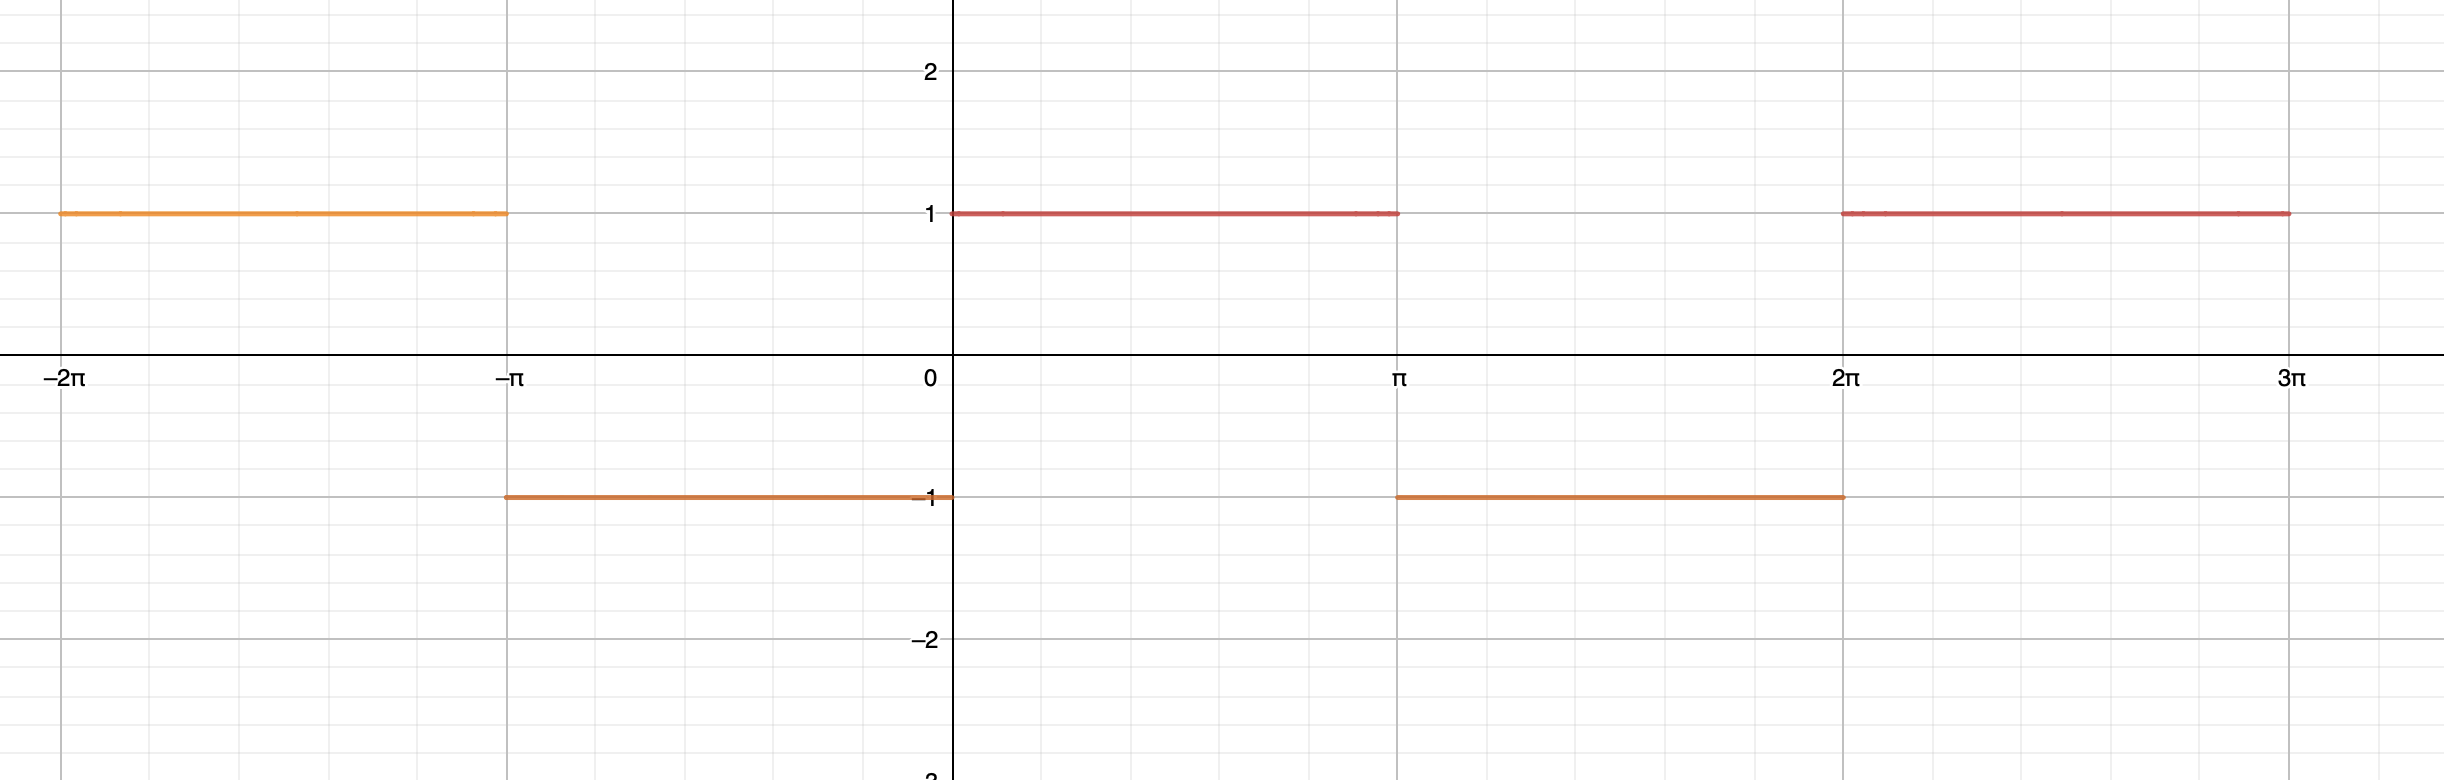
\includegraphics[scale=0.3]{1.png}
\end{center}
$x_0 \in (-\pi, 0) \cup (0, \pi)$, тогда ряд Фурье $\longrightarrow f(x_0)$, а в точках разрыва ($x_0 = -\pi, x_0 = 0, x_0 = \pi$) ряд сходится к полусумме пределов слева и справа, т.е:
\[
\longrightarrow \frac{-1 + 1}{2} = 0 , \text{ тогда ряд Фурье} \longrightarrow 0 
\]
Теперь ищем суммы, начнем с первой:
\[
\sum_{n = 1}^{\infty} \frac{(-1)^{n + 1}}{2n-1}
\]
В полученный ряд подставим $\frac{\pi}{2}$ и получим (слева 1 т.к очев $sign(\frac{\pi}{2}) = 1$):
\[
1 = 
\sum_{n = 1}^{\infty} \frac{4}{\pi(2n - 1)} \cdot \sin(2n -1) \frac{\pi}{2} = \sum_{n = 1}^{\infty} \frac{4}{\pi(2n - 1)} \cdot (-1)^{n + 1} = \frac{4}{\pi} \cdot \sum_{n = 1}^{\infty} \frac{(-1)^{n + 1} }{(2n - 1)}
\]
Ну и отсюда получаем:
\[
\sum_{n = 1}^{\infty} \frac{(-1)^{n + 1} }{(2n - 1)} = \frac{1}{\frac{4}{\pi}} = \frac{\pi}{4}
\]
Теперь ищем вторую:
\[
\sum_{n = 1}^{\infty} \frac{1}{(2n-1)^2}
\]
Для нахождения напишем равенство Парсеваля:
\[
\frac{1}{\pi} \int\limits_{-\pi}^{\pi} sign^2 (x) = \sum_{n = 1}^{\infty} \frac{4^2}{\pi^2 (2n-1)^2}
\]
Считаем левый интеграл:
\[
\frac{1}{\pi} \int\limits_{-\pi}^{\pi} sign^2 (x) = \frac{1}{\pi} \cdot (\pi - (-\pi)) = 2 
\]
То есть:
\[
\sum_{n = 1}^{\infty} \frac{4^2}{\pi^2 (2n-1)^2} = 2
\]
\[
\frac{16}{\pi^2} \cdot \sum_{n = 1}^{\infty} \frac{}{\pi^2 (2n-1)^2} = 2
\]
\[
 \sum_{n = 1}^{\infty} \frac{}{\pi^2 (2n-1)^2} = \frac{\pi^2}{8}
\]
\begin{center}
\textbf{Ответ: } 

разложение:
\[
sign(x) = \sum_{n = 1}^{\infty} \frac{4}{\pi(2n - 1)} \cdot \sin(2n -1) x
\]
cходимость:
\[
x_0 \in (-\pi, 0) \cup (0, \pi), \text{ тогда ряд Фурье} \longrightarrow f(x_0)
\]
\[
x_0 = - \pi, \; x_0 = 0, \;  x_0 = \pi, \text{ тогда ряд Фурье} \longrightarrow 0
\]
суммы:
\[
\sum_{n = 1}^{\infty} \frac{(-1)^{n + 1}}{2n-1} = \frac{\pi}{4}
\]
\[
\sum_{n = 1}^{\infty} \frac{1}{(2n-1)^2} = \frac{\pi^2}{8}
\]
\end{center}
\clearpage
\section*{Номер 2}
Теперь смотрим на $[0, 2\pi]$. График функции есть прямая, которая равна нулю в точке $x = \pi$. Функция нечетная относительно этой точки $\pi$, а значит $a_0 = a_k = 0$. Ищем $b_k$:
\[
b_k = \frac{1}{\pi} \int\limits_0^{2\pi} \left( \frac{\pi - x}{2} \sin kx \right) dx  = \frac{1}{2} \int\limits_0^{2\pi} \sin kx dx - \frac{1}{2\pi} \int\limits_0^{2\pi} x \sin kx dx = (\times)
\]
Считаем отдельно:
\[
\int\limits_0^{2\pi} \sin kx dx = -\frac{\cos kx}{k} \Bigg|_0^{2\pi} = - \frac{\cos 2 \pi k}{k} + \frac{\cos 0}{k} = \frac{2\sin^2 \pi k}{k} = 0
\]
\[
\int\limits_0^{2\pi} x \sin kx dx  = - \frac{x \cos (kx)}{k} \Bigg|_0^{2\pi} + \frac{1}{k} \int\limits_0^{2\pi} \cos(kx) dx  = - \frac{2\pi \cos (2\pi k)}{k} + \frac{\sin (2 \pi k)}{k^2} = - \frac{2\pi}{k}
\]
Подставляем:
\[
(\times) =  - \frac{1}{2\pi} \cdot \left(- \frac{2\pi}{k} \right) =\frac{1}{k}
\]
Итого получаем разложение Фурье:
\[
\frac{\pi - x}{2}  = \sum_{k = 1}^{\infty} \frac{1}{k} \sin (kx) 
\]
Смотрим график:
\begin{center}

\includegraphics[scale=0.3]{2.png}
\end{center}
$x_0 \in(0, 2\pi)$, тогда ряд Фурье $\longrightarrow f(x_0)$, а в точках разрыва $(0, 2\pi)$ ряд сходится к полусумме пределов слева и справа, т.е при $x_0 = 0, x_0 = 2\pi$ ряд Фурье $\longrightarrow 0$.
\\
Теперь ищем суммы, начнем с первой:
\[
\sum_{n = 1}^{\infty} \frac{\sin \left(\pi \frac{n}{3}\right)}{n}
\]
Подставим точку $\frac{\pi}{3}$:
\[
\frac{\pi - \frac{\pi}{3}}{2} = \sum_{n = 1}^{\infty} \frac{1}{n} \sin \left(n\frac{\pi}{3}\right)  = \sum_{n = 1}^{\infty} \frac{\sin \left(\pi \frac{n}{3}\right)}{n}
\]
Ну а значит:
\[
\sum_{n = 1}^{\infty} \frac{\sin \left(\pi \frac{n}{3}\right)}{n} = \frac{\pi}{3}
\]
Смотрим вторую сумму:
\[
\sum_{n = 1}^{\infty} \frac{1}{n^2}
\]
Для нахождения напишем равенство Парсеваля:
\[
\frac{1}{\pi} \int\limits_0^{2\pi}\left( \frac{\pi - x}{2}\right)^2 dx= \sum_{k = 1}^{\infty} \frac{1}{k^2}   = \sum_{n = 1}^{\infty} \frac{1}{n^2}
\]
Найдем интеграл:
\[
\frac{1}{\pi} \int\limits_0^{2\pi}\left( \frac{\pi - x}{2}\right)^2 dx = \frac{1}{4\pi} \int\limits_{0}^{2\pi} (\pi - x)^2 dx = 
\begin{bmatrix}
u = \pi - x \\
du = - dx \\
dx = -du 
\end{bmatrix} =  -\frac{1}{4\pi} 
\int\limits_{\pi}^{-\pi} u^2 du  =
\]
\[
=
-
\frac{1}{4\pi} \cdot \frac{u^3}{3} \Bigg|_{-\pi}^{\pi} =
 -\frac{-\pi^3}{12\pi} + \frac{\pi^3}{12\pi} = \frac{\pi^2}{6}
\]
А значит:
\[
\sum_{n = 1}^{\infty} \frac{1}{n^2} = \frac{\pi^2}{6}
\]
Смотрим третью сумму:
\[
\sum_{n = 1}^{\infty} \frac{(-1)^{n+1}}{2n-1}
\]
Заметим, что в разложении у нас $\sin (kx)$, мы хотим подставить $\frac{\pi}{2}$, чтобы получить $(-1)$ в степени, но тогда синус будет обращаться в ноль при четных $k$, а значит тогда делаем аналогично предыдущему номеру $n = 2 k - 1$ и получаем:
\[
\frac{\pi - \frac{\pi}{2}}{2} = \sum_{n = 1}^{\infty} \frac{1}{2n-1} \sin (2n-1) \frac{\pi}{2} = \sum_{n = 1}^{\infty} \frac{(-1)^{n+1}}{2n-1} 
\]
А значит:
\[
\sum_{n = 1}^{\infty} \frac{(-1)^{n+1}}{2n-1}  = \frac{\pi - \frac{\pi}{2}}{2} = \frac{\pi}{4}
\]
\begin{center}
\textbf{Ответ: } 

разложение:
\[
\frac{\pi - x}{2}  = \sum_{k = 1}^{\infty} \frac{1}{k} \sin (kx) 
\]
cходимость:
\[
x_0 \in(0, 2\pi), \text{ряд Фурье }\longrightarrow f(x_0)
\]
\[
x_0 = 0, x_0 = 2\pi, \text{ряд Фурье }\longrightarrow 0
\]
суммы:
\[
\sum_{n = 1}^{\infty} \frac{\sin \left(\pi \frac{n}{3}\right)}{n} = \frac{\pi}{3}
\]
\[
\sum_{n = 1}^{\infty} \frac{1}{n^2} = \frac{\pi^2}{6}
\]
\[
\sum_{n = 1}^{\infty} \frac{(-1)^{n+1}}{2n-1}  = \frac{\pi}{4}
\]
\end{center}
\end{document}
